% !TeX spellcheck = en_US

\chapter{Software Design}
This chapter discusses the possible solutions for working with GIS inside the LIFE simulation system.



\section{Current state}
Currently the GIS support inside MARS is partial, some components of the environment are capable of handling GIS, while others are not currently supporting it.


\subsection{Web browser Front-end}
The WebUI supports GIS for importing and managing this kind of data. It's successor the teaching UI currently does not support GIS. Due to the micro-service structure of the back-end services it is possible for the front-ends to coexist.

\subsection{Back-end Services}
The back-end services fully support GIS. The file service accepts the uploaded files and hands control over to the GIS Data Service (GDS). 

\subsubsection{GIS Data Service}
The GDS is capable of handling the most common GIS types, these are Geotiff and Esri AsciiGrid for raster and Shapefile for vector files. The files may be provided compressed inside a .zip file or as plain files.\\
During the import the GDS determines the type of data automatically by checking the file extension. Once detected, the file is validated and the spatial reference is determined. In case of a valid geo-referenced input, the file is imported into the GeoServer for persistence.


\subsubsection{GeoServer} \label{sec:GS}
The GeoServer (GS) is an open source software that is tailored to store, manage and share GIS. It offers a web GUI as well as a REST API for interaction. The api is structured in a way that it implements common Open Geospatial Consortium (OGC) standards for retrieving data.\\
The Web Feature Service (WFS) allows to retrieve features of vector data, Web Coverage Service (WCS) enables downloading raster data and the Web Map Service (WMS) can generate a tile map for viewing GIS on a map.\\
The GS is build for working with few files and a small number of users. The MARS use-case requires to read thousands to millions of  single values in parallel in a short amount of time. The GS does not satisfy this demands. The retrieval of single values is not supported, since the general use-case is to work with complete files. The performance for retrieving data is also very poor which will require a better solution.


\subsection{GIS Layer}
The GIS Layer inside MARS LIFE reads the Data provided by the GDS and uses it inside the simulation. Since the migration from C\# to .NET Core inside LIFE the GIS layer is not compatible anymore.\\
The current models therefore do not leverage GIS for their input. Data is being transfered into other formats to work around these shortcomings. Vector data is mainly represented as comma separated values (.csv) files and raster data are represented in custom formats.


\section{Solutions}
As mentioned in section \ref{sec:GS} reading data from the GS during the simulation is not feasible inside a high performance environment.\\
Different alternative solutions have been discovered and evaluated. The data could be stored inside a spatial database that is optimized for parallel reads of single values or the GIS file could be supplied to the Simulation and stored in memory for fast reading. Figure \ref{fig:feature_comparison} shows an overview of the evaluated technologies.

\begin{table}[H]
	\caption{GIS solutions feature comparison}
	\label{fig:feature_comparison}
	\begin{tabular}{|l|l|l|l|}
	\hline \textbf{Name}	& \textbf{Raster support} & \textbf{Vector support} & \textbf{Type}\\
	\hline GeoServer & yes & yes & self-hosted product\\
	\hline PostGIS	& yes* & yes & PostgreSQL DB + GIS ext.\\
	\hline MongoDB	& no & yes & DB with spatial capabilities\\
	\hline Dotspatial & yes & yes & C\# library\\
	\hline NetTopologySuite	& no & yes & C\# library\\
	\hline AsciiGrid Parser & yes & no & Own .NET Core Class\\
	\hline
	\end{tabular}
	\caption*{ \raggedright * Large file failed.}
\end{table}


\subsection{Performance comparison}
All mentioned technologies were tested with the same input files. A small, a medium and a large size vector and raster file. The file sizes were ~10 KB, ~6.5 MB and ~105 MB. Each test performs 1,000 parallel reads and the result is the average of three separate tests. 
The results are listed in figure \ref{fig:vector_performace} for vector and \ref{fig:raster_performace} for raster.

\begin{figure}[H]
	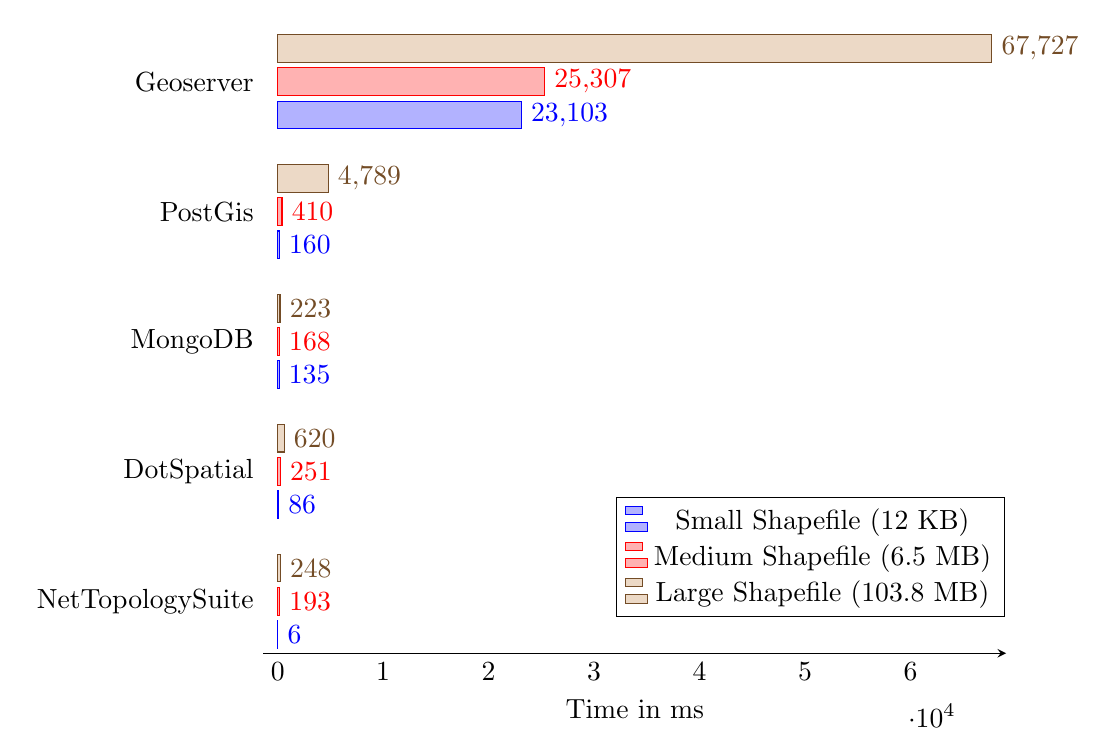
\begin{tikzpicture}
	\begin{axis}[
	xbar,
	y axis line style = { opacity = 0 },
	axis x line       = bottom,
	tickwidth         = 0pt,
	%	enlarge y limits  = 0.02,
	enlarge x limits  = 0.02,
	symbolic y coords = {NetTopologySuite, DotSpatial, MongoDB, PostGis, Geoserver},
	nodes near coords,
	height=9.5cm,
	legend style={at={(0.737,0.25)},anchor=north},
	xlabel={Time in ms},
	]
	% Small Shapefile
	\addplot coordinates {
		(23103,Geoserver)
		(160,PostGis)
		(135,MongoDB)
		(86,DotSpatial)
		(6,NetTopologySuite)
	};
	% Mid Shapefile
	\addplot coordinates {
		(25307,Geoserver)
		(410,PostGis)
		(168,MongoDB)
		(251,DotSpatial)
		(193,NetTopologySuite)
	};
	% Large Shapefile
	\addplot coordinates {
		(67727,Geoserver)
		(4789,PostGis)
		(223,MongoDB)
		(620,DotSpatial)
		(248,NetTopologySuite)
	};
	\legend{Small Shapefile (12 KB),Medium Shapefile (6.5 MB),Large Shapefile (103.8 MB)}
	\end{axis}
	\end{tikzpicture}
	\caption{Vector performance for 1k reads}
	\label{fig:vector_performace}
\end{figure}


\begin{figure}[H]
	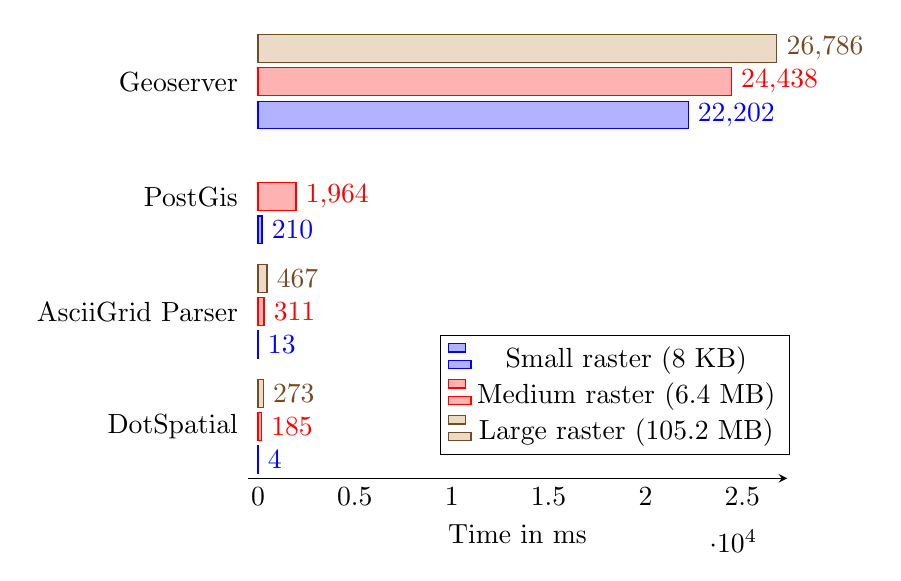
\begin{tikzpicture}
	\begin{axis}[
	xbar,
	y axis line style = { opacity = 0 },
	axis x line       = bottom,
	tickwidth         = 0pt,
	enlarge y limits  = 0.15,
	enlarge x limits  = 0.02,
	symbolic y coords = {DotSpatial, AsciiGrid Parser, PostGis, Geoserver},
	nodes near coords,
	legend style={at={(0.68,0.32)},anchor=north},
	xlabel={Time in ms},
	]
	% Small Rasterfile
	\addplot coordinates {
		(22202,Geoserver)
		(210,PostGis)
		(13,AsciiGrid Parser)
		(4,DotSpatial)
	};
	% Mid Rasterfile
	\addplot coordinates {
		(24438,Geoserver)
		(1964,PostGis)
		(311,AsciiGrid Parser)
		(185,DotSpatial)
	};
	% Large Rasterfile
	\addplot coordinates {
		(26786,Geoserver)
		(nan,PostGis) % 342197
		(467,AsciiGrid Parser)
		(273,DotSpatial)
	};
	\legend{Small raster (8 KB),Medium raster (6.4 MB),Large raster (105.2 MB)}
	\end{axis}
	\end{tikzpicture}
	\caption{Raster performance for 1k reads}
	\label{fig:raster_performace}
\end{figure}


\subsection{PostGIS}
PostGIS is a PostgreSQL with GIS extensions. It supports storing vector data as well as raster data.\\
The performance is way better than the of the GS, however PostGIS did not handle the large file very well. The reading of the large vector file took over 10 times longer than the smaller file, which is surprising since the data is broken into tables. A larger table should not effect the response time by that extend.\\
The big raster file was even worse. The test crashed with an OutOfMemory exception on a machine with 16 GB of RAM. Limiting the parallelism of threads to 7 worked, but the results of around ~340,000 ms (5 min. 40 sec.) were not acceptable.


\subsection{MongoDB}
MongoDB offeres good overall performance for vector data. The file size does not effect the overall performance by a large extend. For the medium and large file it was even faster than NetTopologySuite (NTS). Raster GIS is not supported.


\subsection{DotSpatial}
DotSpatial offers average vector read performance. MongoDB and NTS perform slightly better. Since both these technologies are not available for raster GIS, DotSpatial performes best in that field.\\
As of August 25th 2017 the library has not been ported to .NET Core. This is why an .NET Core compatible Esri AsciiGrid parser was created.\\
The performance measurement for DotSpatial and NTS are different to the database solutions. The way both libraries work is, that they open the file into RAM and read from it. The read performance from RAM for the mentioned scenario is around 0.02 ms for both technologies. Since the file can be loaded once and read from during the simulation, the increased time for additional reads is very low, making these solution preferable.

\subsection{NetTopologySuite}
NTS has the best vector read performance and shares the same RAM based performance benefits as DotSpatial. It is not available for raster GIS. As of August 2017 NTS is available for .NET Core.

\begin{figure}[H]
	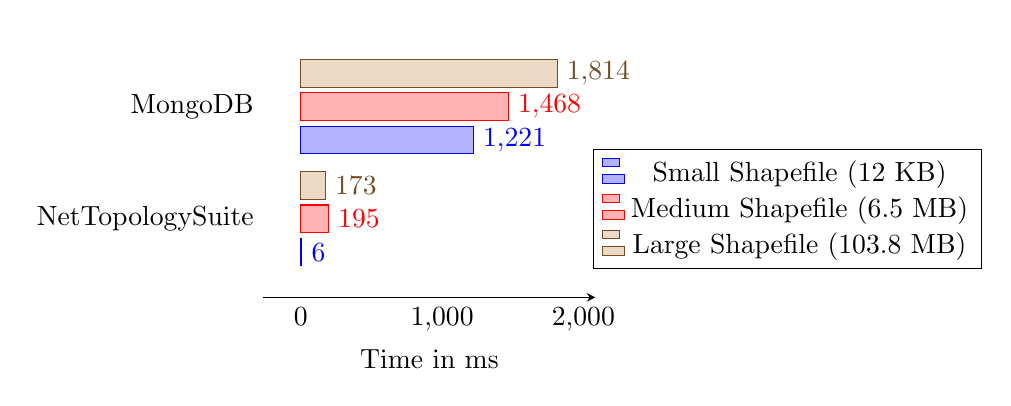
\begin{tikzpicture}
	\begin{axis}[
	xbar,
	y axis line style = { opacity = 0 },
	axis x line       = bottom,
	tickwidth         = 0pt,
	enlarge y limits  = 0.7,
	enlarge x limits  = 0.15,
	symbolic y coords = {NetTopologySuite, MongoDB},
	ytick=data,
	nodes near coords,
	height=5cm,
	legend style={at={(1.58,0.55)},anchor=north},
	xlabel={Time in ms},
	]
	% Small Shapefile
	\addplot coordinates {
		(1221,MongoDB)
		(6,NetTopologySuite)
	};
	% Mid Shapefile
	\addplot coordinates {
		(1468,MongoDB)
		(195,NetTopologySuite)
	};
	% Large Shapefile
	\addplot coordinates {
		(1814,MongoDB)
		(173,NetTopologySuite)
	};
	\legend{Small Shapefile (12 KB),Medium Shapefile (6.5 MB),Large Shapefile (103.8 MB)}
	\end{axis}
	\end{tikzpicture}
	\caption{Vector performance for 10k reads}
	\label{fig:vector_performace_best}
\end{figure}

\begin{figure}[H]
	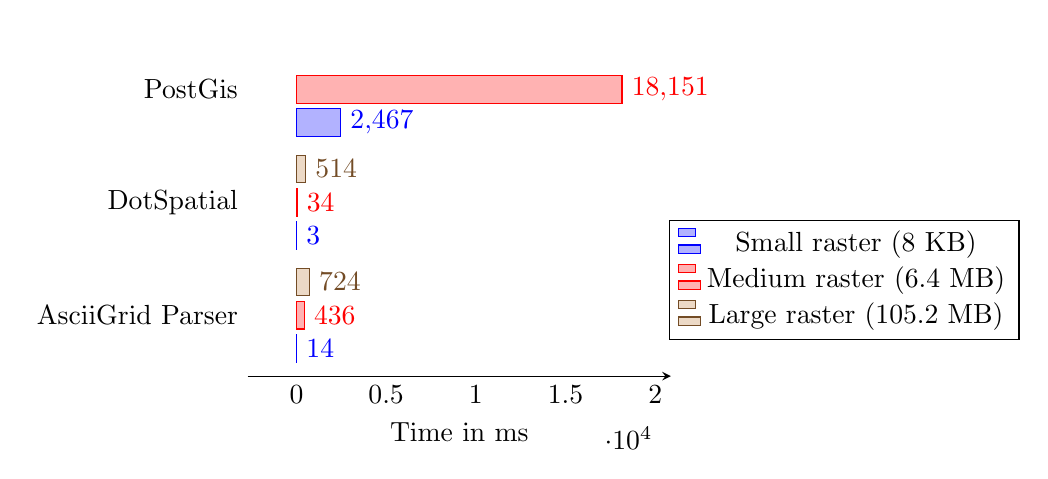
\begin{tikzpicture}
	\begin{axis}[
	xbar,
	y axis line style = { opacity = 0 },
	axis x line       = bottom,
	tickwidth         = 0pt,
	enlarge y limits  = 0.27,
	enlarge x limits  = 0.15,
	symbolic y coords = {AsciiGrid Parser, DotSpatial, PostGis},
	ytick=data,
	nodes near coords,
	height=6cm,
	legend style={at={(1.41,0.45)},anchor=north},
	xlabel={Time in ms},
	]
	% Small Raster
	\addplot coordinates {
		(2467,PostGis)
		(3,DotSpatial)
		(14,AsciiGrid Parser)
	};
	% Mid Raster
	\addplot coordinates {
		(18151,PostGis)
		(34,DotSpatial)
		(436,AsciiGrid Parser)
	};
	% Large Raster
	\addplot coordinates {
		(nan,PostGis)
		(514,DotSpatial)
		(724,AsciiGrid Parser)
	};
	\legend{Small raster (8 KB),Medium raster (6.4 MB),Large raster (105.2 MB)}
	\end{axis}
	\end{tikzpicture}
	\caption{Raster performance for 10k reads}
	\label{fig:raster_performace_best}
\end{figure}


\subsection{AsciiGrid Parser}
Since DotSpatial is not ported to .NET Core yet, there is no acceptable solution for reading raster GIS during the simulation. This is, why the author of this work created a parser for Esri's AsciiGrid format.\\
AsciiGrid is a text-based, geo-referenced raster format that other raster formats like GeoTIFF can be converted into. Due to the text-based nature of the format the read performance is not as good as the DotSpatial reader. It is however acceptable until DotSpatial gets migrated.

